\chapter{कार्बमैग्नीशियम अभिकर्मक}\label{ch:b1:organomagnesium}

अधिकांश उपयोगी कार्बनिक अणुओं में किसी भी सस्ते प्रारंभिक पदार्थ से अधिक
कार्बन परमाणु होते हैं, और संश्लेषण की केंद्रीय समस्या दो कार्बन कंकालों को एक
नए C--C आबंध से जोड़ना है। किसी कार्बन यौगिक में कार्बन लगभग
हमेशा आबंध का इलेक्ट्रॉन-न्यून भागीदार होता है --- ऑक्सीजन के साथ, किसी
हैलोजन के साथ --- और दो इलेक्ट्रॉन-न्यून कार्बन एक-दूसरे से अभिक्रिया नहीं करते।
बीसवीं शताब्दी के आरंभ में एक हैलोऐल्केन और मैग्नीशियम से एक ही फ़्लास्क में बने
एक अभिकर्मक ने इसे उलट दिया: उसका कार्बन इलेक्ट्रॉन-समृद्ध है,
एक \omterm{def:b1:electronic-effects:nucleophile}{नाभिकरागी} जो कार्बोनिल समूह के कार्बन पर आक्रमण करता है। इसकी सहायता से
लगभग किसी भी कंकाल वाले ऐल्कोहॉल छोटे टुकड़ों से बनाए जा सकते हैं। यह
अध्याय दिखाता है कि अभिकर्मक कैसे बनाया जाता है, उसे पूरी तरह शुष्क
फ़्लास्क क्यों चाहिए, वह किससे योग करता है, और उसके साथ योजना कैसे बनाई जाती है।

\begin{recall}
\omterm{def:b1:periodicity:electronegativity}{विद्युत-ऋणात्मकता} (\cref{ch:b1:periodicity}); \omterm{def:b1:lewis-resonance-vsepr:lewis-acid}{लुइस अम्ल} और क्षारक तथा
\omterm{def:b1:lewis-resonance-vsepr:lewis-acid}{उपसहसंयोजी आबंध} (\cref{ch:b1:lewis-resonance-vsepr}); \omterm{def:b1:electronic-effects:nucleophile}{नाभिकरागी},
\omterm{def:b1:electronic-effects:nucleophile}{इलेक्ट्रॉनरागी}, \omterm{def:b1:electronic-effects:curly-arrow}{वक्र तीर} और कार्बनिक स्पीशीज़ का $\mathrm{p}K_a$
पैमाना (\cref{ch:b1:electronic-effects}); किसी ऐल्कोहॉल की श्रेणी
(प्राथमिक, द्वितीयक, तृतीयक) उसके कार्बन की श्रेणी का अनुसरण करती है।
\end{recall}

\section{ग्रीन्यार अभिकर्मक बनाना}

\begin{definition}[कार्बधात्विक यौगिक, ग्रीन्यार अभिकर्मक]\label{def:b1:organomagnesium:organometallic}
\emph{कार्बधात्विक यौगिक}\index{कार्बधात्विक यौगिक} में
कम से कम एक कार्बन--धातु आबंध होता है। \emph{कार्बमैग्नीशियम
यौगिक}\index{कार्बमैग्नीशियम यौगिक} में C--Mg आबंध होता है;
\emph{ग्रीन्यार अभिकर्मक}\index{ग्रीन्यार अभिकर्मक} \ce{RMgX} (X = Cl, Br, I),
जो किसी हैलोऐल्केन या हैलोऐरीन और मैग्नीशियम से किसी ईथर में बनाया जाता है,
\ce{R-X + Mg -> R-MgX}, इनमें सबसे सामान्य है।
\end{definition}

मैग्नीशियम स्वयं को C--X आबंध में प्रविष्ट कर देता है। ईथर कोई
निर्दोष विलायक नहीं है: \ce{RMgX} में मैग्नीशियम के चारों ओर केवल चार \omterm{def:b1:quantum-numbers:configuration}{संयोजकता इलेक्ट्रॉन}
होते हैं, और ईथर के दो अणु उसे अपने \omterm{def:b1:lewis-resonance-vsepr:lewis}{एकाकी युग्म} देते हैं, जिससे
उसका अष्टक पूरा होता है और अभिकर्मक विलयन में बना रहता है।

\begin{omfigure}
\begin{tikzpicture}[font=\small]
  \node (mg) at (0,0) {Mg};
  \node (r) at (-1.5,0) {R};
  \node (x) at (1.5,0) {Br};
  \node (o1) at (0,1.45) {O};
  \node (o2) at (0,-1.45) {O};
  \draw[thick] (r) -- (mg) -- (x);
  \draw[thick, ->, omDef] (o1) -- (mg);
  \draw[thick, ->, omDef] (o2) -- (mg);
  \draw (o1) -- ++(-0.8,0.45) node[left] {\ce{CH3CH2}};
  \draw (o1) -- ++(0.8,0.45) node[right] {\ce{CH2CH3}};
  \draw (o2) -- ++(-0.8,-0.45) node[left] {\ce{CH3CH2}};
  \draw (o2) -- ++(0.8,-0.45) node[right] {\ce{CH2CH3}};
  \node[align=left, anchor=west] at (3.2,0) {ईथर के दो अणु\\एक-एक एकाकी युग्म देते हैं (नीला):\\चतुष्फलकीय मैग्नीशियम,\\इलेक्ट्रॉनों का एक अष्टक};
\end{tikzpicture}

{\small एथॉक्सीएथेन (डाइएथिल ईथर) में एक \omterm{def:b1:organomagnesium:organometallic}{ग्रीन्यार अभिकर्मक}।
ऑक्सीजन--मैग्नीशियम \omterm{def:b1:lewis-resonance-vsepr:lewis-acid}{उपसहसंयोजी आबंध} समझाते हैं कि अभिकर्मक केवल किसी
ईथर या ऐसे ही \omterm{def:b1:lewis-resonance-vsepr:lewis-acid}{लुइस क्षारक} में ही क्यों बनता है।}
\end{omfigure}

\begin{method}[ग्रीन्यार अभिकर्मक बनाना]\label{met:b1:organomagnesium:prepare}
\begin{enumerate}
  \item सारे काँच के उपकरण ओवन में सुखाइए; संघनित्र पर कैल्सियम क्लोराइड की
        शुष्कन नली लगाइए; निर्जल ईथर का उपयोग कीजिए।
  \item मैग्नीशियम की छीलन और थोड़ा ईथर एक तीन-मुखी
        फ़्लास्क में रखिए, जिसमें संघनित्र, योजन कीप और विलोडक लगे हों।
  \item हैलाइड का एक छोटा भाग मिलाइए; जब अभिक्रिया आरंभ हो जाए
        (धुँधलापन, ईथर का हल्का उबलना), शेष को बूँद-बूँद करके
        ऐसी दर से मिलाइए जो हल्का पश्चवाहन बनाए रखे।
  \item विलयन का तुरंत, उसी शुष्क उपकरण में, उपयोग कीजिए।
\end{enumerate}
\end{method}

\begin{omfigure}
\begin{tikzpicture}[font=\small]
  \pic at (0,-0.05) {stirrer};
  \pic (f) at (0,0.05) {threeneck={0.35}{omDef!14}};
  \pic at (f-c) {condenser};
  \pic at ($(f-c)+(0,3.2)$) {guardtube};
  \pic[rotate=25] at (f-l) {dropfunnel={0.5}{orange!20}};
  \fill[black!45, rotate around={-25:(f-r)}] ($(f-r)+(-0.17,0)$) rectangle ++(0.34,0.3);
  \draw[->] (2.4,0.9) node[right] {शुष्क ईथर में Mg की छीलन} -- (0.6,0.6);
  \draw[->] (-3.0,3.9) node[left, align=right] {ईथर में हैलाइड,\\बूँद-बूँद मिलाया गया} -- (-1.8,3.4);
  \draw[->] (1.8,5.3) node[right] {संघनित्र (जल)} -- (0.45,4.8);
  \draw[->] (1.8,6.6) node[right] {कैल्सियम क्लोराइड शुष्कन नली} -- (0.3,6.4);
  \draw[->] (2.4,-0.2) node[right] {चुंबकीय विलोडक} -- (1.3,-0.2);
\end{tikzpicture}

{\small ग्रीन्यार अभिक्रिया का उपकरण: जहाँ तक वायु पहुँच सकती है, वह सब
सुखाया जाता है। वायु की जलवाष्प को शुष्कन नली रोकती है;
संघनित्र उबलते ईथर को फ़्लास्क में लौटा देता है।}
\end{omfigure}

\begin{inthelab}[एक अभिक्रिया जिसे आरंभ होना ही है]
\omterm{def:b1:organomagnesium:organometallic}{ग्रीन्यार अभिकर्मक} बनाना कभी-कभी आरंभ ही नहीं होता: मैग्नीशियम
ऑक्साइड की एक परत से ढका होता है। काँच की छड़ से छीलन के एक टुकड़े को कुचलना,
आयोडीन का एक \omterm{def:b1:crystals-metals:crystal}{क्रिस्टल} मिलाना, या फ़्लास्क को स्थानीय रूप से गरम करना ताज़ी धातु
को खोल देता है। एक बार आरंभ होने पर अभिक्रिया ऊष्माक्षेपी होती है और ईथर अपने आप उबलता है;
तब मिलाना धीमा कर दिया जाता है ताकि वह उफनकर बाहर न निकले। एथॉक्सीएथेन
\qty{35}{\celsius} पर उबलता है और उसकी वाष्प अत्यंत ज्वलनशील है: प्रयोगशाला में
कहीं भी कोई लौ नहीं, और पास में एक बर्फ़-स्नान।
% ledger: bp:diethylether
\end{inthelab}

\section{एक प्रबल क्षारक और एक नाभिकरागी}

\begin{definition}[ध्रुवता प्रतिलोमन]\label{def:b1:organomagnesium:umpolung}
मैग्नीशियम की \omterm{def:b1:periodicity:electronegativity}{विद्युत-ऋणात्मकता} (1.31) कार्बन की (2.55) से बहुत कम है:
\ce{R-MgX} में C--Mg आबंध इस प्रकार ध्रुवित है कि उसका ऋण
सिरा कार्बन पर है, जो \omterm{def:b1:electronic-effects:intermediates}{कार्बऋणायन} की तरह व्यवहार करता है। हैलाइड \ce{R-X} में
वही कार्बन धनात्मक था (X: Br के लिए 2.96)। किसी \omterm{def:b1:electronic-effects:nucleophile}{इलेक्ट्रॉनरागी} कार्बन को
\omterm{def:b1:electronic-effects:nucleophile}{नाभिकरागी} कार्बन में बदलना \emph{ध्रुवता प्रतिलोमन}\index{ध्रुवता प्रतिलोमन} है।
% ledger: en:Mg, en:C, en:Br
\end{definition}

\begin{proposition}[ग्रीन्यार अभिकर्मक अम्लीय हाइड्रोजनों से नष्ट हो जाते हैं]\label{prop:b1:organomagnesium:base}
\omterm{def:b1:organomagnesium:organometallic}{ग्रीन्यार अभिकर्मक} जल, ऐल्कोहॉलों, कार्बोक्सिलिक
अम्लों, N--H आबंध वाले ऐमीनों और अंतस्थ ऐल्काइनों से \omterm{def:b1:extent-q-and-k:quantitative}{मात्रात्मक} रूप से अभिक्रिया करता है, और
ऐल्केन \ce{R-H} देता है: \ce{RMgX + H2O -> R-H + Mg(OH)X}।
\end{proposition}

\begin{proof}
\omterm{def:b1:electronic-effects:intermediates}{कार्बऋणायन} जैसा कार्बन युग्म \ce{R-H}/\ce{R^-} का क्षारक है, और
ऐल्केन कार्बनिक रसायन के अब तक के सबसे \omterm{def:b1:predominant-reaction:strong-acid}{दुर्बल अम्ल} हैं: जल में, जहाँ
हाइड्रॉक्साइड सबसे \omterm{def:b1:predominant-reaction:strong-acid}{प्रबल क्षारक} है जो अस्तित्व में रह सकता है, उनसे किसी प्रोटॉन का निकलना
मापा ही नहीं जा सकता (\cref{ch:b1:predominant-reaction}, समतलन)। सूची का कोई भी अम्ल
बहुत अधिक प्रबल है, और \ce{R^-} को प्रोटॉन स्थानांतरण का
स्थिरांक विशाल है: वह पूर्ण और तीव्र है।
\end{proof}

शुष्क उपकरण का यही कारण है: जल की एक बूँद उतनी ही मात्रा के
अभिकर्मक को नष्ट कर देती है। इसे लाभ में बदलें, तो \ce{CH3CH2MgBr + D2O}
ठीक वहीं एक ड्यूटेरियम परमाणु रख देता है जहाँ ब्रोमीन था।

\section{कार्बोनिल यौगिकों और कार्बन डाइऑक्साइड पर योग}

C=O समूह का कार्बन \omterm{def:b1:electronic-effects:nucleophile}{इलेक्ट्रॉनरागी} है
(\cref{ch:b1:electronic-effects})। \omterm{def:b1:organomagnesium:organometallic}{ग्रीन्यार अभिकर्मक} अपना R समूह
उससे जोड़ता है, और C=O का $\pi$ युग्म ऑक्सीजन पर चला जाता है; फिर अम्लीय उपचार
ऐल्कॉक्साइड को प्रोटॉनित करता है।

\begin{omfigure}
\setchemfig{atom sep=2.1em}
\schemestart
\chemfig{@{r}R-[@{rm}]MgBr}
\+
\chemfig{@{cc}C(-[:150]R')(-[:210]R'')=[@{co}]@{o}O}
\arrow{->}
\chemfig{C(-[:150]R')(-[:210]R'')(-[2]R)-O^{-}}
\chemfig{\phantom{.}}\chemfig{^{+}MgBr}
\arrow{->[\ce{H3O+}]}
\chemfig{C(-[:150]R')(-[:210]R'')(-[2]R)-OH}
\schemestop
\chemmove{\draw[->, thick, shorten <=2pt, shorten >=2pt](rm) .. controls +(70:9mm) and +(180:7mm) .. (cc);
          \draw[->, thick, shorten <=2pt, shorten >=2pt](co) .. controls +(90:6mm) and +(90:6mm) .. (o);}
\par\vspace{6pt}

{\small किसी कीटोन (या ऐल्डिहाइड,
$\mathrm{R''} = \mathrm{H}$) पर \omterm{def:b1:organomagnesium:organometallic}{ग्रीन्यार अभिकर्मक} का योग: C--Mg युग्म नया C--C आबंध बनाता है जबकि C=O का $\pi$
युग्म ऑक्सीजन पर जाता है; मैग्नीशियम ऐल्कॉक्साइड तनु अम्ल द्वारा
एक अलग चरण में प्रोटॉनित होता है।}
\end{omfigure}

\begin{proposition}[कार्बोनिल यौगिकों से ऐल्कोहॉल]\label{prop:b1:organomagnesium:carbonyl-addition}
अम्लीय उपचार के बाद, \omterm{def:b1:organomagnesium:organometallic}{ग्रीन्यार अभिकर्मक} \ce{RMgX} देता है: मेथेनल के साथ, एक
प्राथमिक ऐल्कोहॉल \ce{RCH2OH}; किसी अन्य ऐल्डिहाइड $\mathrm{R'CHO}$ के साथ, एक द्वितीयक
ऐल्कोहॉल $\mathrm{RR'CHOH}$; किसी कीटोन $\mathrm{R'COR''}$ के साथ, एक तृतीयक ऐल्कोहॉल
$\mathrm{RR'R''COH}$। नया C--C आबंध R को पूर्व कार्बोनिल कार्बन से जोड़ता है।
\end{proposition}

\begin{proof}
कार्बोनिल कार्बन अपने दो प्रतिस्थापी बनाए रखता है और R तथा एक OH
(ऐल्कॉक्साइड ऑक्सीजन से) प्राप्त करता है: मेथेनल दो H लाता है, ऐल्डिहाइड एक H और
एक कार्बन समूह, कीटोन दो कार्बन समूह। ऐल्कोहॉल की श्रेणी
उस कार्बन पर कार्बन समूहों की संख्या है: एक, दो या तीन।
\end{proof}

\begin{proposition}[कार्बन डाइऑक्साइड से कार्बोक्सिलिक अम्ल]\label{prop:b1:organomagnesium:co2}
ठोस कार्बन डाइऑक्साइड पर उँडेला गया \omterm{def:b1:organomagnesium:organometallic}{ग्रीन्यार अभिकर्मक},
अम्लीकरण के बाद, एक अधिक कार्बन वाला कार्बोक्सिलिक अम्ल \ce{RCOOH} देता है:
\ce{RMgX + CO2 -> RCOOMgX}, फिर \ce{RCOOMgX + H3O+ -> RCOOH + Mg^2+ + X- + H2O}।
\end{proposition}

\begin{proof}
\ce{CO2} एक कार्बोनिल यौगिक है जिसके कार्बन पर कीटोन के कार्बन की तरह
आक्रमण होता है; बना हुआ कार्बोक्सिलेट इन परिस्थितियों में दूसरा R समूह जोड़ने के लिए
बहुत अनभिक्रियाशील है (ऋणावेशित कार्बोनिल एक दुर्बल
\omterm{def:b1:electronic-effects:nucleophile}{इलेक्ट्रॉनरागी} है)। अम्ल उसे प्रोटॉनित करता है।
\end{proof}

\section{कार्बन कंकालों का निर्माण}

\begin{method}[किसी ऐल्कोहॉल की योजना]\label{met:b1:organomagnesium:plan-alcohol}
\begin{enumerate}
  \item लक्ष्य ऐल्कोहॉल में OH वहन करने वाला कार्बन खोजिए।
  \item उसके कार्बन समूहों में से एक को R चुनिए (वह
        \omterm{def:b1:organomagnesium:organometallic}{ग्रीन्यार अभिकर्मक} से आएगा, जो \ce{R-Br} से बनाया जाता है); अणु का
        शेष भाग, उस कार्बन को C=O के रूप में लेकर, कार्बोनिल भागीदार है।
  \item संभावित विकल्पों (प्रति कार्बन समूह एक) की सूची बनाइए और उस विकल्प को
        वरीयता दीजिए जिसके अभिकर्मक सरल और उपलब्ध हों।
  \item जाँचिए कि किसी भी भागीदार पर अम्लीय हाइड्रोजन या दूसरा
        कार्बोनिल न हो जो वह भी अभिक्रिया करे।
\end{enumerate}
\end{method}

\begin{example}[2-फ़ेनिलब्यूटेन-2-ऑल]\label{ex:b1:organomagnesium:plan}
OH वहन करने वाले कार्बन पर एक फ़ेनिल, एक मेथिल और एक एथिल समूह है।
तीन विकल्प: ब्यूटेन-2-ओन के साथ फ़ेनिलमैग्नीशियम ब्रोमाइड; 1-फ़ेनिलप्रोपेन-1-ओन के साथ
मेथिलमैग्नीशियम ब्रोमाइड; 1-फ़ेनिलएथेन-1-ओन (ऐसीटोफ़ीनोन) के साथ
एथिलमैग्नीशियम ब्रोमाइड। तीनों काम करते हैं; अंतिम में दो
सबसे सामान्य अभिकर्मक प्रयुक्त होते हैं।
\end{example}

\begin{history}[विक्टर ग्रीन्यार]
\begin{minipage}[t]{0.2\linewidth}\vspace{0pt}
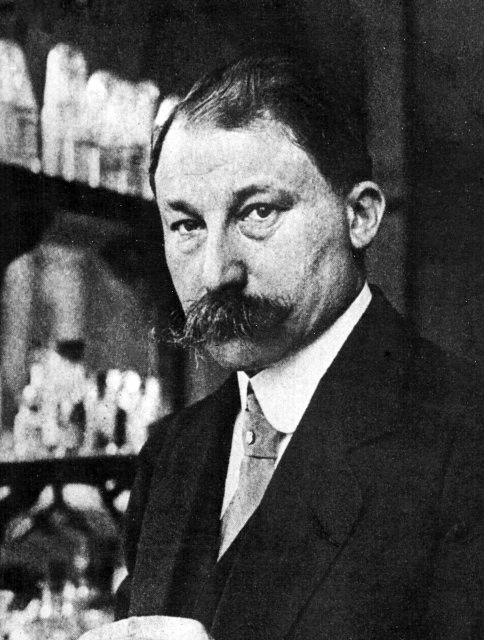
\includegraphics[width=\linewidth]{images/book2/grignard.jpg}
\end{minipage}\hfill
\begin{minipage}[t]{0.76\linewidth}\vspace{0pt}
यह अभिकर्मक विक्टर ग्रीन्यार के नाम से जाना जाता है, जिन्होंने बीसवीं शताब्दी के
आरंभ में एक शोध-छात्र के रूप में पाया कि मैग्नीशियम किसी हैलोऐल्केन के
ईथर विलयन में घुल जाता है और वह विलयन कार्बोनिल यौगिकों से
योग करता है। इसकी सरलता --- एक धातु, एक विलायक, एक फ़्लास्क
--- ने इसे शताब्दी की सबसे अधिक प्रयुक्त कार्बन--कार्बन आबंध बनाने वाली
अभिक्रिया बना दिया, और इसके खोजकर्ता को रसायन का नोबेल पुरस्कार दिलाया।
(छायाचित्र, सार्वजनिक अधिकार-क्षेत्र, विकिमीडिया कॉमन्स।)
\end{minipage}
\end{history}

\section{अभ्यास}

\begin{exercise}[$\star$]\label{exo:b1:organomagnesium:1}
एथिलमैग्नीशियम ब्रोमाइड और फ़ेनिलमैग्नीशियम ब्रोमाइड बनाने की
अभिक्रियाएँ लिखिए। \omterm{def:b1:periodicity:electronegativity}{विद्युत-ऋणात्मकताओं} के साथ C--Br आबंध और C--Mg आबंध का
ध्रुवण बताइए।
\end{exercise}

\begin{exercise}[$\star$]\label{exo:b1:organomagnesium:2}
मेथिलमैग्नीशियम आयोडाइड इनके साथ क्या देता है: जल; एथेनॉल; एथेनोइक
अम्ल; ड्यूटेरियम ऑक्साइड \ce{D2O}? समीकरण लिखिए।
\end{exercise}

\begin{exercise}[$\star$]\label{exo:b1:organomagnesium:3}
मेथेनल, एथेनल, प्रोपेनोन, बेंज़ैल्डिहाइड और कार्बन डाइऑक्साइड के साथ
एथिलमैग्नीशियम ब्रोमाइड का उत्पाद (अम्लीय उपचार के बाद) बताइए। हर
ऐल्कोहॉल की श्रेणी बताइए।
\end{exercise}

\begin{exercise}[$\star$]\label{exo:b1:organomagnesium:4}
\omterm{def:b1:organomagnesium:organometallic}{ग्रीन्यार अभिकर्मक} बनाने के लिए 4-ब्रोमोब्यूटेन-1-ऑल का उपयोग क्यों नहीं करना चाहिए?
\end{exercise}

\begin{exercise}[$\star\star$]\label{exo:b1:organomagnesium:5}
एथेनल पर मेथिलमैग्नीशियम ब्रोमाइड के योग की
और उपचार की क्रियाविधि \omterm{def:b1:electronic-effects:curly-arrow}{वक्र तीरों} के साथ लिखिए। क्या उत्पाद \omterm{def:b1:stereochemistry-in-depth:stereocentre}{किरैल} है? क्या वह
एक अकेले \omterm{def:b1:stereochemistry-in-depth:enantiomers}{प्रतिबिंबरूपी} के रूप में मिलता है? क्यों?
\end{exercise}

\begin{exercise}[$\star\star$]\label{exo:b1:organomagnesium:6}
किसी \omterm{def:b1:organomagnesium:organometallic}{ग्रीन्यार अभिकर्मक} और किसी कीटोन से 3-मेथिलपेंटेन-3-ऑल बनाने के दो ढंग
प्रस्तावित कीजिए।
\end{exercise}

\begin{exercise}[$\star\star$]\label{exo:b1:organomagnesium:7}
2-ब्रोमोप्रोपेन से आप 2-मेथिलप्रोपेनोइक अम्ल कैसे बनाएँगे?
\qty{70}{\percent} \omterm{def:b1:extent-q-and-k:fractional-extent}{लब्धि} पर \qty{12.3}{g} ब्रोमाइड से प्राप्त अम्ल का द्रव्यमान
परिकलित कीजिए ($M$: \ce{C3H7Br} \qty{123.0}{g/mol}, \ce{C4H8O2}
\qty{88.0}{g/mol})।
\end{exercise}

\begin{exercise}[$\star\star$]\label{exo:b1:organomagnesium:8}
एक लापरवाह विद्यार्थी \qty{0.18}{g} जल युक्त ईथर में
\qty{0.0500}{mol} ब्रोमोबेंज़ीन से फ़ेनिलमैग्नीशियम ब्रोमाइड बनाता है।
अभिकर्मक का कितना अंश नष्ट होता है? कौन-सा उत्पाद बनता है?
\end{exercise}

\begin{exercise}[$\star\star$]\label{exo:b1:organomagnesium:9}
बाइफ़ेनिल, \ce{C6H5-C6H5}, फ़ेनिलमैग्नीशियम ब्रोमाइड बनाने में एक उपोत्पाद है।
प्रस्तावित कीजिए कि यह कैसे बनता है, और आधिक्य मैग्नीशियम में
ब्रोमोबेंज़ीन को धीरे-धीरे मिलाना इसे सीमित क्यों करता है।
\end{exercise}

\begin{exercise}[$\star\star\star$]\label{exo:b1:organomagnesium:10}
किसी \omterm{def:b1:organomagnesium:organometallic}{ग्रीन्यार अभिकर्मक} से 1-फ़ेनिलएथेन-1-ऑल के दो संश्लेषणों की, और
2-फ़ेनिलप्रोपेन-2-ऑल के एक संश्लेषण की योजना बनाइए। हर एक के लिए वह हैलाइड बताइए जो
अभिकर्मक देता है।
\end{exercise}

\begin{exercise}[$\star\star\star$]\label{exo:b1:organomagnesium:11}
समझाइए कि \omterm{def:b1:organomagnesium:organometallic}{ग्रीन्यार अभिकर्मक} और कार्बोनिल यौगिक को नीचे की
समस्या में चुने गए क्रम में ही क्यों मिलाना चाहिए, और उपचार केवल जल के बजाय
ठंडे तनु अम्ल से क्यों किया जाता है।
\end{exercise}

\begin{exercise}[$\star\star\star$]\label{exo:b1:organomagnesium:12}
किसी ब्रोमाइड के \qty{0.100}{mol} से बने \omterm{def:b1:organomagnesium:organometallic}{ग्रीन्यार अभिकर्मक} का \omterm{def:b1:titration-methods:titration}{अनुमापन} किया जाता है:
एक भाग को आधिक्य जल में उँडेला जाता है, और बने क्षारकीय मैग्नीशियम लवण का
हाइड्रोक्लोरिक अम्ल से \omterm{def:b1:titration-methods:titration}{अनुमापन} किया जाता है: पूरे विलयन के अनुपात में,
\qty{0.088}{mol} अम्ल लगता है। सिद्धांत समझाइए और बनाने की \omterm{def:b1:extent-q-and-k:fractional-extent}{लब्धि}
बताइए।
\end{exercise}

\section{समस्या: ट्राइफ़ेनिलमेथेनॉल}

\begin{problem}[{सप्ताहांत समस्या --- फ़ेनिलमैग्नीशियम ब्रोमाइड बनाना,
बेंज़ोफ़ीनोन पर उसका योग, उपचार, और
ट्राइफ़ेनिलमेथेनॉल की लब्धि}]
\label{pb:b1:organomagnesium:1}
एक शुष्क तीन-मुखी फ़्लास्क में \qty{0.535}{g} मैग्नीशियम और
\qty{3.14}{g} ब्रोमोबेंज़ीन निर्जल एथॉक्सीएथेन में
फ़ेनिलमैग्नीशियम ब्रोमाइड देते हैं। फिर उसी ईथर में \qty{3.28}{g} बेंज़ोफ़ीनोन,
\ce{(C6H5)2CO}, का विलयन बूँद-बूँद करके मिलाया जाता है। ठंडे तनु सल्फ़्यूरिक अम्ल से
उपचार, निष्कर्षण और पुनःक्रिस्टलन के बाद,
\qty{3.75}{g} शुद्ध ट्राइफ़ेनिलमेथेनॉल, \ce{(C6H5)3COH}, प्राप्त होता है,
और \qty{0.15}{g} बाइफ़ेनिल पृथक किया जाता है। मोलर द्रव्यमान (\unit{g/mol}):
Mg 24.3, \ce{C6H5Br} 156.9, \ce{C13H10O} 182.0, \ce{C19H16O} 260.0,
\ce{C12H10} 154.0, \ce{C7H6O2} 122.0।

\medskip
\noindent\textbf{भाग I --- फ़ेनिलमैग्नीशियम ब्रोमाइड।}
\begin{enumerate}
  \item बनाने का समीकरण लिखिए।
  \item मैग्नीशियम और ब्रोमोबेंज़ीन की मात्राएँ परिकलित कीजिए। कौन-सा
        आधिक्य में है?
  \item उपकरण शुष्क क्यों होना चाहिए? जल के साथ अभिक्रिया लिखिए।
  \item शुष्कन नली की क्या भूमिका है?
  \item अभिकर्मकों को घोलने के अतिरिक्त, ईथर अनिवार्य क्यों है?
  \item बाइफ़ेनिल अभिकर्मक की ब्रोमोबेंज़ीन से अभिक्रिया से आता है।
        इसे लिखिए और इसमें खोई ब्रोमोबेंज़ीन की मात्रा परिकलित कीजिए।
\end{enumerate}

\medskip
\noindent\textbf{भाग II --- योग।}
\begin{enumerate}[resume]
  \item बेंज़ोफ़ीनोन की मात्रा परिकलित कीजिए।
  \item योग की क्रियाविधि \omterm{def:b1:electronic-effects:curly-arrow}{वक्र तीरों} के साथ लिखिए।
  \item कौन-सा अभिकर्मक ट्राइफ़ेनिलमेथेनॉल के बनने को सीमित करता है? भाग I को
        ध्यान में रखिए।
  \item क्या ट्राइफ़ेनिलमेथेनॉल \omterm{def:b1:stereochemistry-in-depth:stereocentre}{किरैल} है? औचित्य दीजिए।
  \item बेंज़ोफ़ीनोन को अभिकर्मक में क्यों मिलाया जाता है, उलटा क्यों नहीं?
  \item बेंज़ोफ़ीनोन विलयन में जल का अंश मात्र क्या करेगा?
\end{enumerate}

\medskip
\noindent\textbf{भाग III --- उपचार।}
\begin{enumerate}[resume]
  \item ऐल्कॉक्साइड का प्रोटॉनन लिखिए।
  \item केवल जल के बजाय ठंडे तनु अम्ल का उपयोग क्यों?
  \item ईथर से निष्कर्षण के बाद ट्राइफ़ेनिलमेथेनॉल और मैग्नीशियम लवण
        कहाँ हैं?
  \item बाइफ़ेनिल को ट्राइफ़ेनिलमेथेनॉल से कैसे पृथक किया जाता है? (बाइफ़ेनिल ठंडे
        हल्के पेट्रोलियम में कहीं अधिक विलेय है।)
  \item कौन-सा परीक्षण \omterm{def:b1:crystals-metals:crystal}{क्रिस्टलों} की शुद्धता की पुष्टि करता है?
  \item ट्राइफ़ेनिलमेथेनॉल ठंडे तनु अम्ल में बचा रहता है, पर
        सांद्र सल्फ़्यूरिक अम्ल में घुलकर गहरा पीला \omterm{def:b1:electronic-effects:intermediates}{कार्बधनायन} देता है।
        उसका बनना लिखिए और उसके स्थायित्व की व्याख्या कीजिए
        (\cref{ch:b1:electronic-effects} से तुलना कीजिए)।
\end{enumerate}

\medskip
\noindent\textbf{भाग IV --- \omterm{def:b1:extent-q-and-k:fractional-extent}{लब्धि}, और एक अन्य उत्पाद।}
\begin{enumerate}[resume]
  \item प्राप्त ट्राइफ़ेनिलमेथेनॉल की मात्रा परिकलित कीजिए।
  \item सीमांत अभिकर्मक के सापेक्ष \omterm{def:b1:extent-q-and-k:fractional-extent}{लब्धि} परिकलित कीजिए।
  \item हानि के दो कारण सुझाइए।
  \item यदि भाग I का अभिकर्मक (बाइफ़ेनिल के लिए संशोधित) इसके बजाय ठोस
        कार्बन डाइऑक्साइड पर उँडेला गया होता, तो कौन-सा उत्पाद बनता?
  \item उस उत्पाद का सैद्धांतिक द्रव्यमान परिकलित कीजिए।
  \item उस कार्बोक्सिलन का समीकरण लिखिए।
  \item ट्राइफ़ेनिलमेथेनॉल की \omterm{def:b1:extent-q-and-k:fractional-extent}{लब्धि} प्रतिशत में बताइए।
\end{enumerate}
\end{problem}
